\section{Complex numbers}

\begin{frame}
\frametitle{Complex numbers}
\begin{columns}
	\begin{column}{0.5\textwidth}
		\begin{definition}
			$j = \sqrt{-1}$
		\end{definition}
		\begin{block}{Cartesian form}
			x= a + b j\\
			$\Re(x) = a$ \quad $\Im(x) = b$
		\end{block}
		\begin{block}{Polar form}
			$x = Re^{\theta j}$\\
			$R = \sqrt{a^2+b^2}$ \qquad $\theta = \arctan(\frac{b}{a})$
		\end{block}
	\end{column}
	\begin{column}{0.5\textwidth}
		\begin{figure}
			\centering
			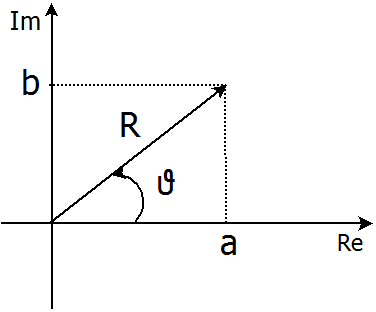
\includegraphics[width=1\linewidth]{Images/afbeelding_4}
		\end{figure}

	\end{column}
\end{columns}

\end{frame}

\begin{frame}
\frametitle{Complex numbers}

	\begin{columns}
		\begin{column}{0.4\textwidth}
		\begin{block}{How many zero's has $x^n-1$?}
			\begin{center}
					\begin{align*}
					x^6 &=  1\\
					x^6 & = e^{2 k \pi j}\\
					x &= e^{\frac{k \pi}{3}j} \\
					x &= \{1,e^{\frac{\pi}{3}j},e^{\frac{2\pi}{3}j},-1,\\
					& \qquad  e^{\frac{4\pi}{3}j},e^{\frac{5\pi}{3}j}\}
					\end{align*}
			\end{center}
		\end{block}
		\end{column}
		\begin{column}{0.6 \textwidth}
			\begin{figure}
			\centering
		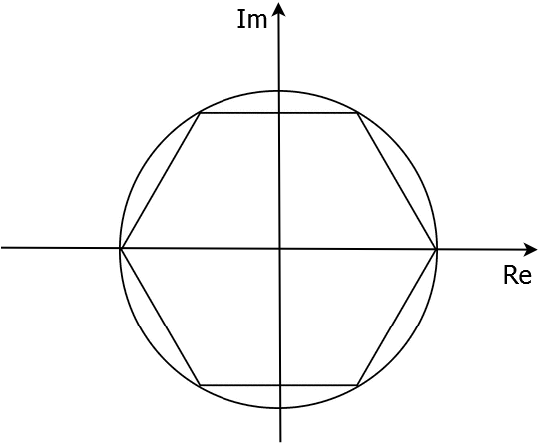
\includegraphics[width=1\linewidth]{Images/afbeelding5}

		\end{figure}

		\end{column}
	\end{columns}
\end{frame}
\begin{frame}
	\frametitle{Complex numbers}
	\begin{block}{How to calculate power of complex number?}
			\begin{align*}
				(a+b j)^n &=R (cos(\theta) + sin(\theta) j ) \\
				& = \big(Re^{\theta j}\big)^{n} \\
				& = R^n e^{n \theta j} \\
				& = R^n (\cos(n \theta) + \sin(n \theta)j) 
			\end{align*}
	\end{block}
\end{frame}
\begin{frame}
	\frametitle{Complex conjugate}
	\begin{definition}
		The conjugate of a complex number is the complex number with same real part and an opposite imaginary part.
		$\overline{a+bj} = a-bj$
	\end{definition}
	Product of 2 complex conjugate numbers result in a complex number with only a real part.\\
	$(a + bj)(a-bj) = a^2 - abj + abj + b^2= a^2 +b^2$\\
	\begin{block}{Dividing complex numbers}
			$\frac{a+bj}{c+dj} = \frac{(a+bj)(c-dj)}{(c^2+d^2)}$\\
			Alternative:\\
			$\frac{a+bj}{c+dj} = \frac{R_1 e^{j\theta_1}}{R_2 e^{j \theta_2}} = \big(\frac{R_1}{R_2}\big) e^{j(\theta_1-\theta_2)}$
	\end{block}

\end{frame}